% Figure s04f02_gauge (Session 4): the Peierls phases of one field in two gauges.
% The image is rendered by figures/blender/s04f02_gauge.py; the coordinates of the labels come from
% figures/blender/out/s04f02_gauge_anchors.tex. Build with figures/blender/build_figure.sh s04f02_gauge.
\documentclass[11pt,tikz,border=0pt]{standalone}
\usepackage[T1]{fontenc}
\usepackage{amsmath,amssymb,graphicx,bm}
\usepackage{xcolor}
\usetikzlibrary{arrows.meta,calc}
% The three label colors of the figures, with the same values as in src/figures_preamble.tex.
\definecolor{aqmaccent}{RGB}{31,78,121}
\definecolor{aqmbroken}{RGB}{168,42,34}
\definecolor{aqmmuted}{RGB}{125,125,125}

\newlength{\figw}\setlength{\figw}{12.5cm}   % 0.8 of the text width

\begin{document}
\begin{tikzpicture}[lbl/.style={font=\small, inner sep=1.5pt}, pnl/.style={font=\small\bfseries, inner sep=1.5pt}]
  \node[anchor=south west, inner sep=0pt] at (0,0)
    {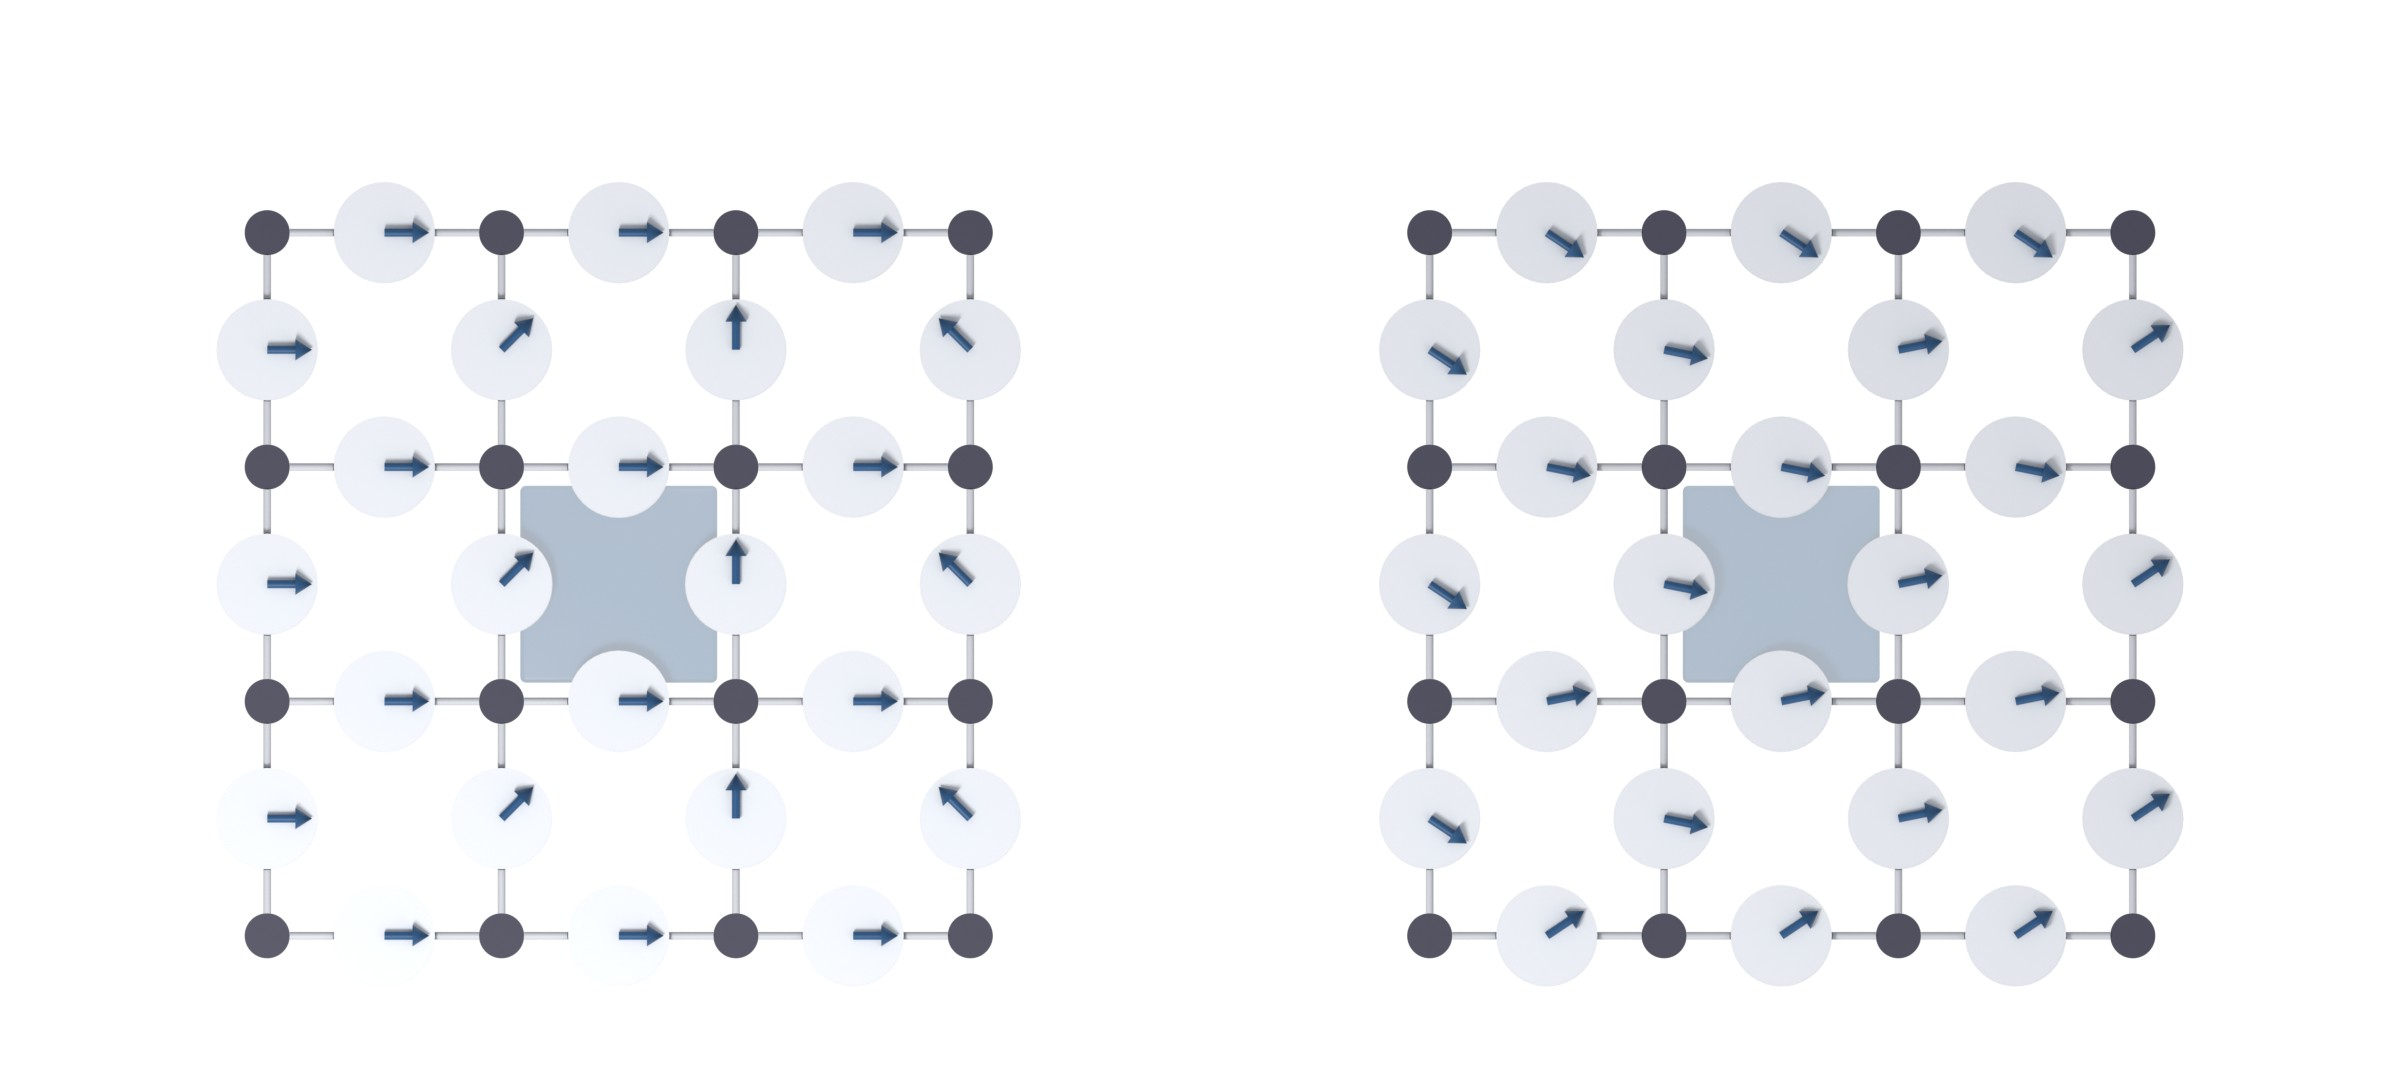
\includegraphics[width=\figw]{../blender/out/s04f02_gauge.jpg}};
  %% written by figlib.py; x and y in units of the image width
\coordinate (apanel) at (0.0840\figw,0.3861\figw);
\coordinate (aplaq) at (0.2578\figw,0.2045\figw);
\coordinate (bpanel) at (0.5684\figw,0.3861\figw);
\coordinate (bplaq) at (0.7422\figw,0.2045\figw);

  \node[lbl, anchor=south west] at (apanel) {\textbf{(a)}\quad Landau gauge};
  \node[lbl, anchor=south west] at (bpanel) {\textbf{(b)}\quad symmetric gauge};
  \node[lbl, text=aqmaccent] at (aplaq) {$\varphi$};
  \node[lbl, text=aqmaccent] at (bplaq) {$\varphi$};
\end{tikzpicture}
\end{document}
